\documentclass[11pt]{article}

%%%%%%%%%%%%%%Include Packages%%%%%%%%%%%%%%%%%%%%%%%%%%
\usepackage{xcolor}
\usepackage{mathtools}
\usepackage[a4paper, total={6in, 8in}, margin=1.25in]{geometry}
\usepackage{amsmath}
\usepackage{amssymb}
\usepackage{paralist}
\usepackage{rsfso}
\usepackage{amsthm}
\usepackage{wasysym}
\usepackage[inline]{enumitem}   
\usepackage{hyperref}
\usepackage{tocloft}
\usepackage{titlesec}
\usepackage{colortbl}
\usepackage{wrapfig}
\usepackage{pdfpages}
%%%%%%%%%%%%%%%%%%%%%%%%%%%%%%%%%%%%%%%%%%%%%%%%%%%%%%%%



\begin{document}
%\begin{wrapfigure}[9]{r}{0.3\textwidth}
%  \begin{center}
%  \vspace{-15pt}
%    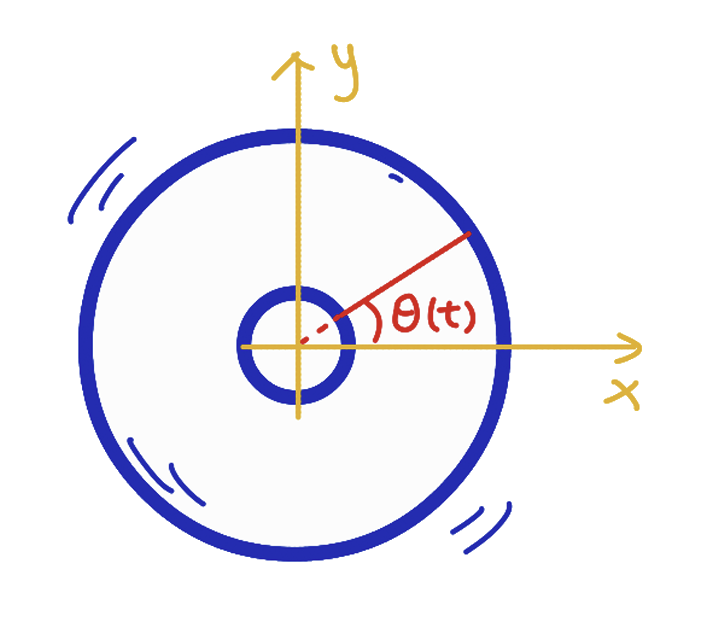
\includegraphics[scale=0.19]{disk}
%  \end{center}
%\end{wrapfigure}
\Large \noindent \textbf{Physics 1A Discussion (Week 9)}\\
\normalsize
Department of Physics and Astronomy, UCLA\\
\noindent\rule{8cm}{0.4pt}\\
Consider two boxes connected by a massless rope, via a \underline{massless} pulley. Box $A$ on the table has a weight of $90$\,N, and box $B$ hanging from the rope has a weight of $25$\,N. The table has a coefficient of kinetic friction $\mu_k = 5/9$.
\begin{center}
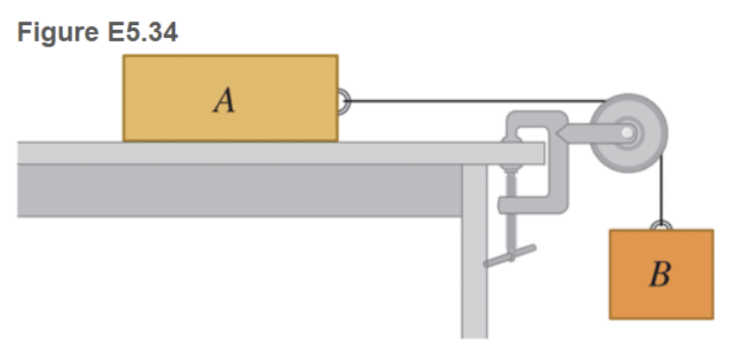
\includegraphics[scale=0.39]{boxes.png}
\end{center}
Once box $B$ is set into downward motion, box $A$ is found to experience an acceleration $a = -2.13$ m/s$^2$ (moving to the right but slowing down). We have seen this problem before (week-4 discussion worksheet, solution on BruinLearn), and the way we previously solved for the acceleration of the system is by setting up a system of equations: one equation ($\vec{F}_{\text{net}} = m\vec{a}$) for each box, 
\begin{align*}
\begin{cases}
-\mu_k m_A g +F_T = m_A a\\
F_T - m_B g = -m_B a\end{cases} \,,
\end{align*}
from which we get $a = -2.13$ m/s$^2$. \\

\noindent Now suppose the pulley, with radius $R$, \underline{does have a mass $M$}, nothing else gets changed. We set box $B$ again into some initial downward motion. \\

\noindent \textbf{(a)} Find the acceleration of box $A$. \\

\noindent \textbf{(b)} Using the expression obtained from part (a), show that $a$ approaches $-2.13$ m/s$^2$ when $M$ approaches zero, so we get back to the case of having the massless pulley. \\

\noindent \textbf{(c)} Find the tensions on box $A$ and box $B$. Why are they not equal?\\

\noindent \textbf{(d)} Suppose $M=1$\,kg. Find the magnitude of the force of the table on the pulley. \\

\vfill
\noindent Hint:
\color{gray}
For part (a), use $\tau = I \alpha$ for the pulley to set up a system of equations. 
\color{black}\\
\noindent Double Hint:
\color{gray}
For part (c), think about what the pulley is doing here. 
\color{black}\\
\noindent Triple Hint:
\color{gray}
For part (d), note that the pulley has no translational motion.
\color{black}


\newpage
\textbf{Solutions}: To find the acceleration of the system, we proceed very similarly to what we have done in the week-4 discussion sheet (review the solution if needed). The net force acting on box $A$ has only the $x$-component being non-zero, thus, taking rightward motion to be positive for box $A$,
\begin{align*}
m_A a = -\mu_k m_A g +F_{T,A}\,,
\end{align*}
which is very similar to what we obtained for box $A$ in the massless-pulley case. The only difference is the $F_{T,A}$ which is the tension force acting on box $A$ by the rope, and we have no information about whether the magnitude of the tension on $A$ is the same as that on $B$, thus we include a subscript in $F_{T,A}$ indicating that this is the tension acting on $A$. Similarly, we write down Newton's second law for the vertical motion of box $B$, upward being the positive direction,
\begin{align*}
 -m_B a = F_{T,B} - m_B g \,.
\end{align*}
Notice the negative sign in front of $m_{B}a$, that comes from the fact that, when $A$ accelerates to the right (giving a positive $a$), $B$ has to be accelerating downwards ($a$ is positive, so a negative sign is added manually). \\

So far, everything is similar to what we have done in week 4, as if the pulley has no mass. Now the pulley does have a mass, so it takes some effort to make it to spin according to $tau = I \alpha$, where $I = (1/2) MR^2$ for this pulley. When box $A$ is accelerating to the right, the pulley must spin clockwise faster and faster, so the angular acceleration of the pulley is related to the linear acceleration of the boxes, by 
\begin{align*}
\alpha = \frac{a}{R}\,.
\end{align*}
Here I have taken clockwise direction to be positive angular acceleration (in contrast with the convention where counterclockwise is positive, but this is fine, as long as we keep everything consistent). This relation is obtained by considering the linear acceleration of the rim on the pulley, which is accelerating together with box $A$ by an amount of $a$, so the angular acceleration of the pulley is $a/R$ with $R$ being the radius of the pulley. Next, there are two forces contribute to the torque acting on the pulley, which are the tension force pulling the pulley to the left (connected to box $A$), and the tension force pulling the pulley down (connected to box $B$), therefore, 
\begin{align*}
\tau_{\text{net}} = -RF_{T,A} +RF_{T,B} 
\end{align*}
for the net torque acting on the pulley, where again I have taken clockwise spinning to be positive. Using the ``Newton's second law" for rotation, $\tau = I\alpha$, we obtain the third equation in our system, 
\begin{align*}
-RF_{T,A} +RF_{T,B} = \frac{MR^2}{2} \frac{a}{R}\,.
\end{align*}
Thus we have a system of three equations, 
\begin{align*}
\begin{cases}
m_A a = -\mu_k m_A g +F_{T,A}\,,\\
 -m_B a = F_{T,B} - m_B g\,,\\
 -RF_{T,A} +RF_{T,B} = MR a/2\,.
\end{cases}
\end{align*}
For a sanity check, we have three unknowns in this problem, $F_{T,A}$, $F_{T,B}$, and $a$. Everything else we can find a number in the problem to plug in (or leave them as variables, namely $M$ and $R$). Solving this system of equations, we obtain 
\begin{align*}
a= -\frac{50\cdot 9.81}{230+9.81 M}\,,\qquad
F_{T,A} = 50 -\frac{50\cdot 90}{230+9.81 M}\,,\qquad
F_{T,B} = 25 -\frac{50\cdot 25}{230+9.81 M}\,.
\end{align*}
The unit for acceleration is m/s$^2$ and the unit for the forces is N. Notice that the final result does not depend on the radius of the pulley. \\

\noindent Taking $M \to 0$, we find
\begin{align*}
a = -\frac{50 \cdot 9.81}{230} = -2.13\,\text{m/s}^2\,,
\end{align*}
as expected.\\

The tensions on box $A$ and $B$ have been found above, notice that they are generally not equal (when we plug a some number for $M$) because of the presence of the pulley. The section of the rope between the pulley and box $B$ has only one tension, which is in general not equal to that of the section of the rope between the pulley and box $A$. These two tensions are both ``spinning" the pulley - contribute to the net torque on the pulley. \\

Finally, talking about the forces acting on the pulley. We have talked about two forces acting on the pulley, tension $F_{T,A}$ to the left, and tension $F_{T,B}$ downwards. In addition to these two, we have two more forces acting on the pulley, which are the force by the table, and the gravitational force. Now we sum all of them together, by Newton's second law, they sum to zero because the pulley has zero translational motion, 
\begin{align*}
-F_{T,A}\hat{x} -F_{T,B}\hat{y}-Mg \hat{y} +\vec{F}_{\text{table}}   = \vec{F}_{\text{net}} = M\vec{a}_{\text{pulley}}= 0
\end{align*}
This allows us to calculate the magnitude of $\vec{F}_{\text{table}}$, 
\begin{align*}
|\vec{F}_{\text{table}}| = \sqrt{F_{T,A}^2 + (F_{T,B} + Mg)^2 } = 50.8\,\text{N}\,.
\end{align*}


\end{document}


